\documentclass[10pt,xcolor=pdflatex]{beamer}
\usepackage{newcent}
\usepackage[utf8]{inputenc}
%\usepackage[czech]{babel}
\usepackage{hyperref}
\usepackage{fancyvrb}
\usetheme{FIT}

%%%%%%%%%%%%%%%%%%%%%%%%%%%%%%%%%%%%%%%%%%%%%%%%%%%%%%%%%%%%%%%%%%
\title[Short Title]{Automatizované testování systému Fitcrack}

\author[]{Juraj Chripko}

\institute[]{Brno University of Technology, Faculty of Information Technology\\
Bo\v{z}et\v{e}chova 1/2. 612 66 Brno - Kr\'alovo Pole\\
login@fit.vutbr.cz}

%\date{January 26, 2018}
\date{\today}
%\date{} % bez data

%%%%%%%%%%%%%%%%%%%%%%%%%%%%%%%%%%%%%%%%%%%%%%%%%%%%%%%%%%%%%%%%%%

\begin{document}

\frame[plain]{\titlepage}

\begin{frame}\frametitle{BOINC a Hashcat}
	\begin{itemize}
		\item Volunteer computing
		\item Grid computing
		\item Správa klientov
		\item Hashcat
	\end{itemize}
    %Example \emph{content}.
\end{frame}

\begin{frame}\frametitle{Fitcrack}
	\begin{figure}[h]
		\centering
		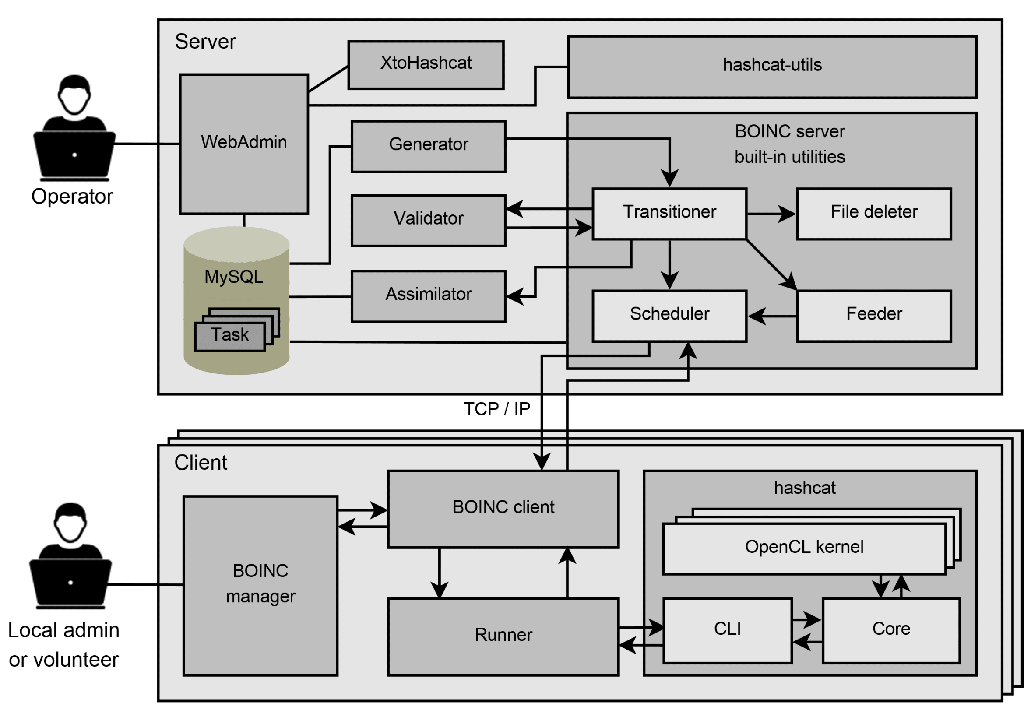
\includegraphics[width=10cm]{img/fc_arch-1.png}
		\caption{Architektúra systému Fitcrack~\cite{TR_TARZAN}.}
		\label{fig:fc_arch}
	\end{figure}
\end{frame}

\begin{frame}\frametitle{Návrh testov pre systém Fitcrack}
	\begin{itemize}
		\item \emph{Integračné testy}
			\begin{itemize}
				\item REST API $\rightarrow$  serverový modul
			\end{itemize}
		\item \emph{Jednotkové testy}
			\begin{itemize}
				\item Generátor
				\item Runner
			\end{itemize}
	\end{itemize}
\end{frame}


\bibliographystyle{plain}
\begin{thebibliography}{99}
	\bibitem[Technická zpráva]{TR_TARZAN}Hranický, R.; Zobal, L.; Večeřa: Distribuovaná obnova hesel. \newblock \emph{Technická zpráva}, \textbf{2017}, \newblock URL \url{http://www.fit.vutbr.cz/research/view_pub.php.cs?id=11568}
\end{thebibliography}

\end{document}
